\pagestyle{fancy}
\fancyfoot[R]{Aron, Amareldo, Aldo}
Die Werte, die von den Messkisten geschickt werden, werden in einem Datenbank gespeichert. Jede Kiste hat einen eigenen ID, Raum, wo sie ist und die MAC-Adresse der Raspberry PI. Die server-seitige Programmierung wird mit PHP gemacht und der client-seitige Programmierung (die Website) mit HTML,CSS f\"ur Design der Website und PHP, die uns hilft, die Website mit dem Webserver kommunizieren zu k\"onnen. S
	\section{Website}
	\section{Datenbankdesign}
	Eine Datenbank wird erstellt, die auf einem Webserver l\"auft. Der Server wird mithilfe einer Raspberry PI simuliert. Der Server hat eine statische IP-Adresse und muss 24 Stunden online sein. Die Verbindung mit der Datenbank wird \"uber WLAN durchgef\"uhrt. Sehen Sie auf die Abb. \ref{fi:ERD}
	\subsection{Struktur der Datenbank}
	Die Datenbank hat zwei Tabellen. Die Tabellen werden mit einem Fremdschl\"ussel miteinander verbunden. Die erste Tabelle hei{\ss}t Messkiste. Diese Tabelle hat 4 Spalten. 
	\begin{itemize}
		\item Die erste Spalte ist 'ID', mit der die Messkiste identifiziert wird. ID ist unique und jede Messkiste hat eine eigene ID. Die ID wird selbst f\"ur jede neue Messkiste um eins erh\"oht. Datentyp von ID ist 'int' und darf keine Null-Werte haben. 
		\item Die zweite Spalte ist 'Raum', die einen Datentyp varchar(50) hat. Das bedeutet, dass Name des Raumes muss maximum 50 Buchstaben enthalten. Jede Messkiste hat einen Taster. Wenn sie montieren werden, wird dieser Taster gedr\"uckt und wird in der Website gezeigt, dass der Taster dieser Messkiste mit diesem ID ist gedr\"uckt und wird gespeichert, in welchem Raum die Messkiste ist.
		\item Die dritte Spalte ist 'Status'. In dieser Spalte wird gespeichert, ob die Messkiste mit der Datenbank verbunden ist. 
		\item Die vierte Spalte ist 'MAC-Adresse'. Der Datentyp von dieser Spalte ist varchar(12). MAC-Adresse ist von Raspberry PI. In der Datenbank werden die Bindestriche von MAC-Adresse nicht gespeichert z.B. 'AABBCCDDEEFF'.
		\begin{figure}
			\centering
			\label{fi:ERD}
			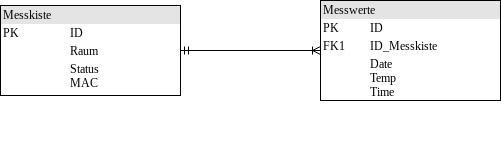
\includegraphics[scale=0.7]{./bilder/db.png}
			\caption{ERD-Diagramm}
		\end{figure} 
		
		\end{itemize}
	\\
	Die zweite Tabelle hei{\ss}t 'Messwerte' und hat 5 Spalten. Diese Tabelle wird mit der ersten Tabelle durch einen Fremdschl\"ussel verbundet.
	\begin{itemize}
		\item Die erste Spalte ist 'ID', mit der die Messwert identifiziert wird. ID ist unique und jede Messkiste hat eine eigene ID. Die ID wird selbst f\"ur jede neue Messkite um eins erh\"oht. Datentyp von ID ist 'int' und darf keine Null-Werte haben. 
	\end{itemize}